\documentclass[8pt]{article} 

% Formatting:
% -----------------------------------------------------------------------------------------------
\setlength{\oddsidemargin}{0cm} 
\setlength{\topmargin}{0cm}
\setlength{\textheight}{21cm}
\setlength{\textwidth}{16.0cm}
\setlength{\columnwidth}{16.0cm} 

% Packages:
% -----------------------------------------------------------------------------------------------
\usepackage[intlimits]{amsmath}
\usepackage{amssymb}
\usepackage{amsfonts}
\usepackage{amsthm}
\usepackage{latexsym}
\usepackage{epsfig}
\usepackage{color}
\usepackage{float}
\usepackage{graphicx}
\usepackage{fancyhdr}
\usepackage{lipsum} 
\usepackage{listings}

\usepackage{array}
\usepackage{booktabs}
\usepackage{courier}
\usepackage{mdframed}
\usepackage{pgfgantt}
\usepackage{rotating}
\usepackage{titling}
\usepackage{url}
\usepackage{verbatim}
\usepackage[margin=50pt,font=small,labelfont=bf]{caption}

\usepackage{pdfpages}
\graphicspath{figures}
%\usepackage{relsize}
%\usepackage{tikz}

%listings stuff
% -----------------------------------------------------------------------------------------------
\lstset{basicstyle=\footnotesize\ttfamily,breaklines=true}
%\lstset{framextopmargin=50pt,frame=bottomline}
\lstset{framextopmargin=50pt}


% Table Shit from Bidski
% ------

\newcolumntype{L}[1]{>{\raggedright\let\newline\\\arraybackslash\hspace{0pt}}m{#1\textwidth}}
\newcolumntype{C}[1]{>{\centering\let\newline\\\arraybackslash\hspace{0pt}}m{#1\textwidth}}
\newcolumntype{R}[1]{>{\raggedleft\let\newline\\\arraybackslash\hspace{0pt}}m{#1\textwidth}}

% Theorem environments:
% -----------------------------------------------------------------------------------------------
\newtheorem{thm}{Theorem}
\newtheorem{prp}{Proposition}
\newtheorem{cor}{Corollary}
\newtheorem{lem}{Lemma}
\newtheorem{df}{Definition}
\newtheorem{alg}{Algorithm}
\newtheorem{con}{Conjecture}

\graphicspath {figs/} 

\pdfpagewidth 8.5in
\pdfpageheight 11in

\pagestyle{fancy}

\lhead{COMP3851A - CompSci Work Integrated Learning Part A}
\chead{}
\rhead{Project Plan Report}
%\rfoot{Right bottom}
\cfoot{\thepage}
%\lfoot{Left bottom}

% Commands
% -----------------------------------------------------------------------------------------------
\newcommand{\inftyint}{\int_{-\infty}^{+\infty}}
\newcommand{\unit}[1]{\ensuremath{\, \mathrm{#1}}}

\newcommand{\executeiffilenewer}[3]{%
\ifnum\pdfstrcmp{\pdffilemoddate{#1}}%
{\pdffilemoddate{#2}}>0%
{\immediate\write18{#3}}\fi%
}
\newcommand{\includesvg}[1]{%
\executeiffilenewer{#1.svg}{#1.pdf}%
{inkscape -z -D --file=#1.svg %
--export-pdf=#1.pdf --export-latex}%
\input{#1.pdf_tex}%
}

% -----------------------------------------------------------------------------------------------



\begin{document}
\numberwithin{equation}{section}

%
% ---- TITLE ------------------------------------------------------------------------------------
% -----------------------------------------------------------------------------------------------
%

%      %%%
%     %%%%
%    %%%%%
%   %%%%%%
%      %%%
%      %%%
%      %%%
%      %%%
%      %%%
%      %%%
%   %%%%%%%%%
%   %%%%%%%%%
%
%
% ---- INTRODUCTION -----------------------------------------------------------------------------
% -----------------------------------------------------------------------------------------------
%

\title{
	
\includegraphics[scale=0.5]{UON_Logo}
	\vspace{60pt}
	\\COMP3851A - CompSci Work Integrated Learning Part A
	\\ \textbf {Remote Control Car learns to drive using Machine Learning}
	\\ \textbf {Project Plan }  
}
\author{
	Jordan Haigh (c3256730), Evan Gresham (c3196094), Mathew Rixon (c3274723) \\
	The University of Newcastle, Australia\\
}
%\date{Last Revision: \today}
% -----------------------------------------------------------------------------------------------


\maketitle

\newpage

%      %%%%%
%    %%%%%%%%%
%   %%%     %%%
%           %%%
%           %%%
%      %%%%%%%
%    %%%%%%%
%   %%%
%   %%%
%   %%%
%   %%%%%%%%%%%
%   %%%%%%%%%%%
%
%
% -----------------------------------------------------------------------------------------------
%

\section{Summary}
Self driving cars are no longer a thing of the future, we have them here and now, however the Artificial intelligence in these vehicles requires thousands of hours of training data and millions of lines of code, where the developers directly teach the the AI how to act. Our team believes this to be excessively onerous. During this project our team intends to have a car learn to drive all by itself, through the process of trial and error. The only difference between us and Tesla is that the cars we will be working on are slightly smaller.  
\\\\
The team will attach a Raspberry Pi to a remote control car and have it learn to drive using current methods in reinforcement learning. The team will also deliver a virtual simulation of the car which will allow us to easily implement and compare multiple popular algorithms in machine learning.

\section {Background}
\subsection{Robotics}
The AI industry focuses on processing information from the environment, tools like image classifiers and speed translators are commonplace. We are interested in using AI to interact back with the environment, like self-driving cars and robotics.

\subsection{Artificial Intelligence and Reinforcement Learning}
We are interested in AI and it's applications in robotics. Each member has completed a Machine Intelligence course at UON, which provided insight into different types of AI, and their possibilities.
\\\\
We will implement and compare different methods and types of AI, such as Q-learning, Deep learning, and Evolutionary algorithms. 

\subsection{Self-Driving Cars}
Self-driving cars are a huge focus for AI, it is to the degree that these cars are completely autonomous. The automation technology has progressed a long way, from Cruise Control\cite{CruiseControl} in 1984, to the fully AI controlled driving with Google Waymo\cite{WaymoProject} in 2009. And from there it's only been getting better.

\subsection{Problems in the Area}
The main problem with modern AI is whether the implementations are able to generalise beyond their training. Some argue that the world is too variable for AI to cope, and so this generalisation will be a focus of our research.

\newpage


%
% -----------------------------------------------------------------------------------------------
%

%      %%%%%
%    %%%%%%%%%
%   %%%     %%%
%           %%%
%           %%%
%      %%%%%%%
%      %%%%%%%
%           %%%
%           %%%
%   %%%     %%%
%    %%%%%%%%%
%      %%%%%
%
%
% -----------------------------------------------------------------------------------------------
%

\section{Aims / Expected Outcomes}

\subsection{Aims}
\begin{itemize}
	\item Create a simulated environment in software to closely resemble the real world functionality of the selected vehicle.
	\begin{itemize}
		\item Accurately model the vehicle and its behaviour.
		\item Build a virtual track to test the vehicle on.
		\item Simulate required physics to allow for an accurate simulation of the motion of the vehicle.
	\end{itemize}

	\item Implement Machine Learning and Artificial Intelligence algorithms in the simulated environment.
	\begin{itemize}
		\item Condition-Based Algorithm
		\item Evolutionary Algorithm
		\item Q-learning
		\item Deep Q-learning
	\end{itemize}

	\item Compare and contrast current algorithms in Machine Learning and Artificial Intelligence based on their performance and efficiency.

	\item Select the most appropriate algorithm to implement in the real world RC Car example

	\item Interface a Raspberry Pi with the selected remote control vehicle to allow intelligent control of the vehicle.

	\item Add required sensors to the Raspberry Pi. e.g. ultrasonic distance sensor, accelerometer.

	\item Implement the chosen Machine Learning algorithm on the Raspberry Pi controlling the vehicle.
	
	\item Construct a physical track from materials which is easily modifiable, cheap and sturdy.  
	
	\item Have a remote control car drive autonomously around a physical track utilising learned behavior.
\end{itemize}

\subsection{Expected Outcomes}
 The team will deliver a program which accurately simulates the movement of the chosen RC car. This program will control the car using a selection of AI algorithms - some AIs will operate through learned actions, other AIs will exhibit preprogramed behaviour. 
\\\\
An RC Car will also be delivered which is controlled by an attached Raspberry Pi; this will perceive the environment through multiple distance sensors. A chosen AI algorithm will be implemented on the Raspberry Pi to control the car, allowing it to navigate through the environment.


\subsection{Team Experience / Skills}
This project requires the team to implement a series of AI algorithms, connect a Raspberry Pi to an RC car and sensors, and build a simulation of the RC car in a 3D environment. The team is confident in our ability to achieve these aims due to previous experience in:

\begin{itemize}
	\item Implementing all mentioned AI algorithms
	\item Controlling hardware with Raspberry Pis
	\item Creating 3D environments in Physics/ Game engines
	
\end{itemize}
We have also allocated time during this project for learning additional skills and programs.

\section{Activity Plan / Timetable}
Our group will place emphasis on creating a software solution in conjunction with the creation a hardware solution. Each team member will have their own tasks and deadlines; some tasks will require collaborative work to meet deadlines. Each member will be involved in the production of hardware / software solution.
\\\\
Gantt Charts have been created for both semesters outlining the tasks that need to be completed and expected deadlines. Each task has been allocated generous time, though there is an option to push back work to the second semester as a last resort.

%      %%%%%
%    %%%%%%%%%
%   %%%     %%%
%   %%%     %%%
%   %%%     %%%
%   %%%     %%%
%    %%%%%%%%%%
%      %%%%% %%
%           %%%
%   %%%     %%%
%    %%%%%%%%%
%      %%%%%
%
%
% -----------------------------------------------------------------------------------------------
%



\begin{figure}
	\centering
	
	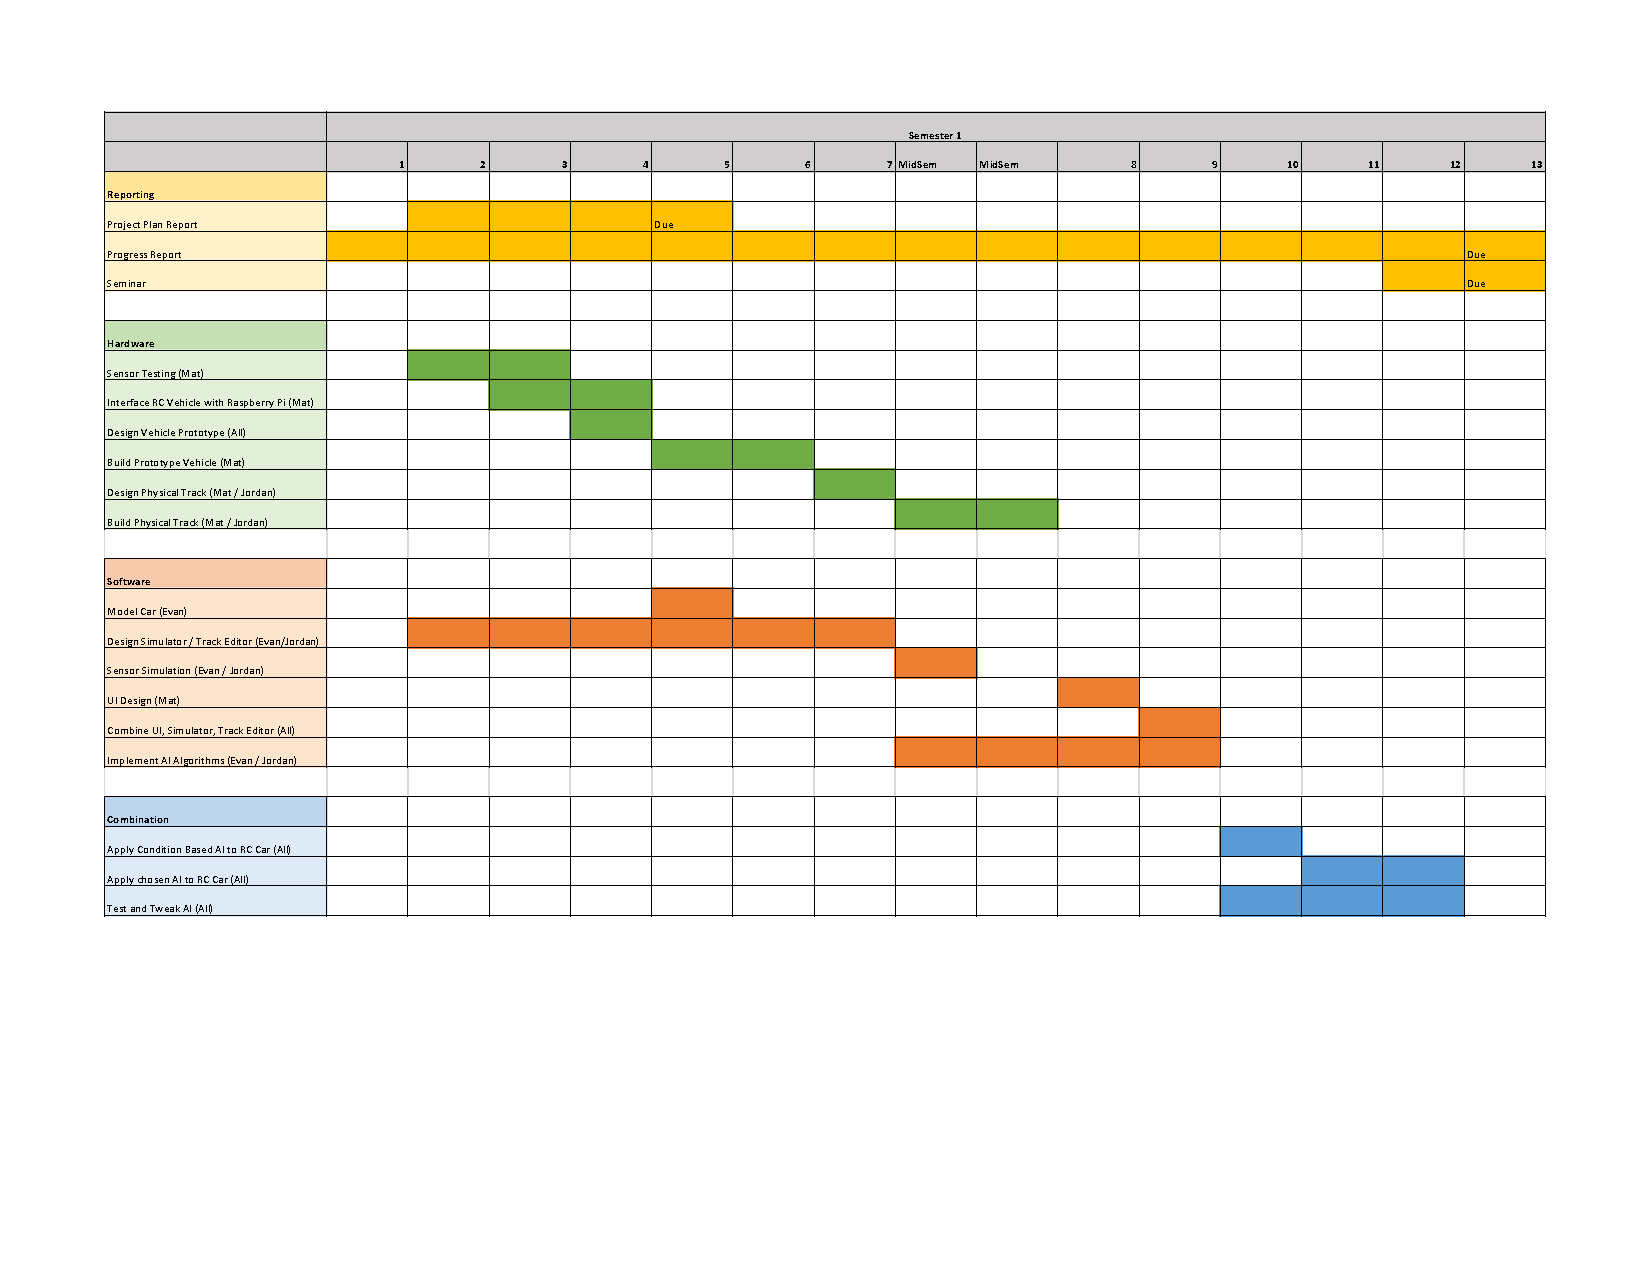
\includegraphics[width=23cm, height = 20cm, angle=90]{figures/TimelineSem1_2_Culled.pdf}
	\caption{Expected Timeline for Semester 1}
\end{figure}




%      %%%  	    %%%%%
%     %%%%		  %%%%%%%%%
%    %%%%%		 %%%     %%%
%   %%%%%%		 %%%     %%%
%      %%%		 %%%     %%%
%      %%%		 %%%     %%%
%      %%%		 %%%     %%%
%      %%%		 %%%     %%%
%      %%%		 %%%     %%%
%      %%%		 %%%     %%%
%   %%%%%%%%%	  %%%%%%%%%
%   %%%%%%%%%	    %%%%%
%
%
% -----------------------------------------------------------------------------------------------
%
\begin{figure}
	\centering
	
	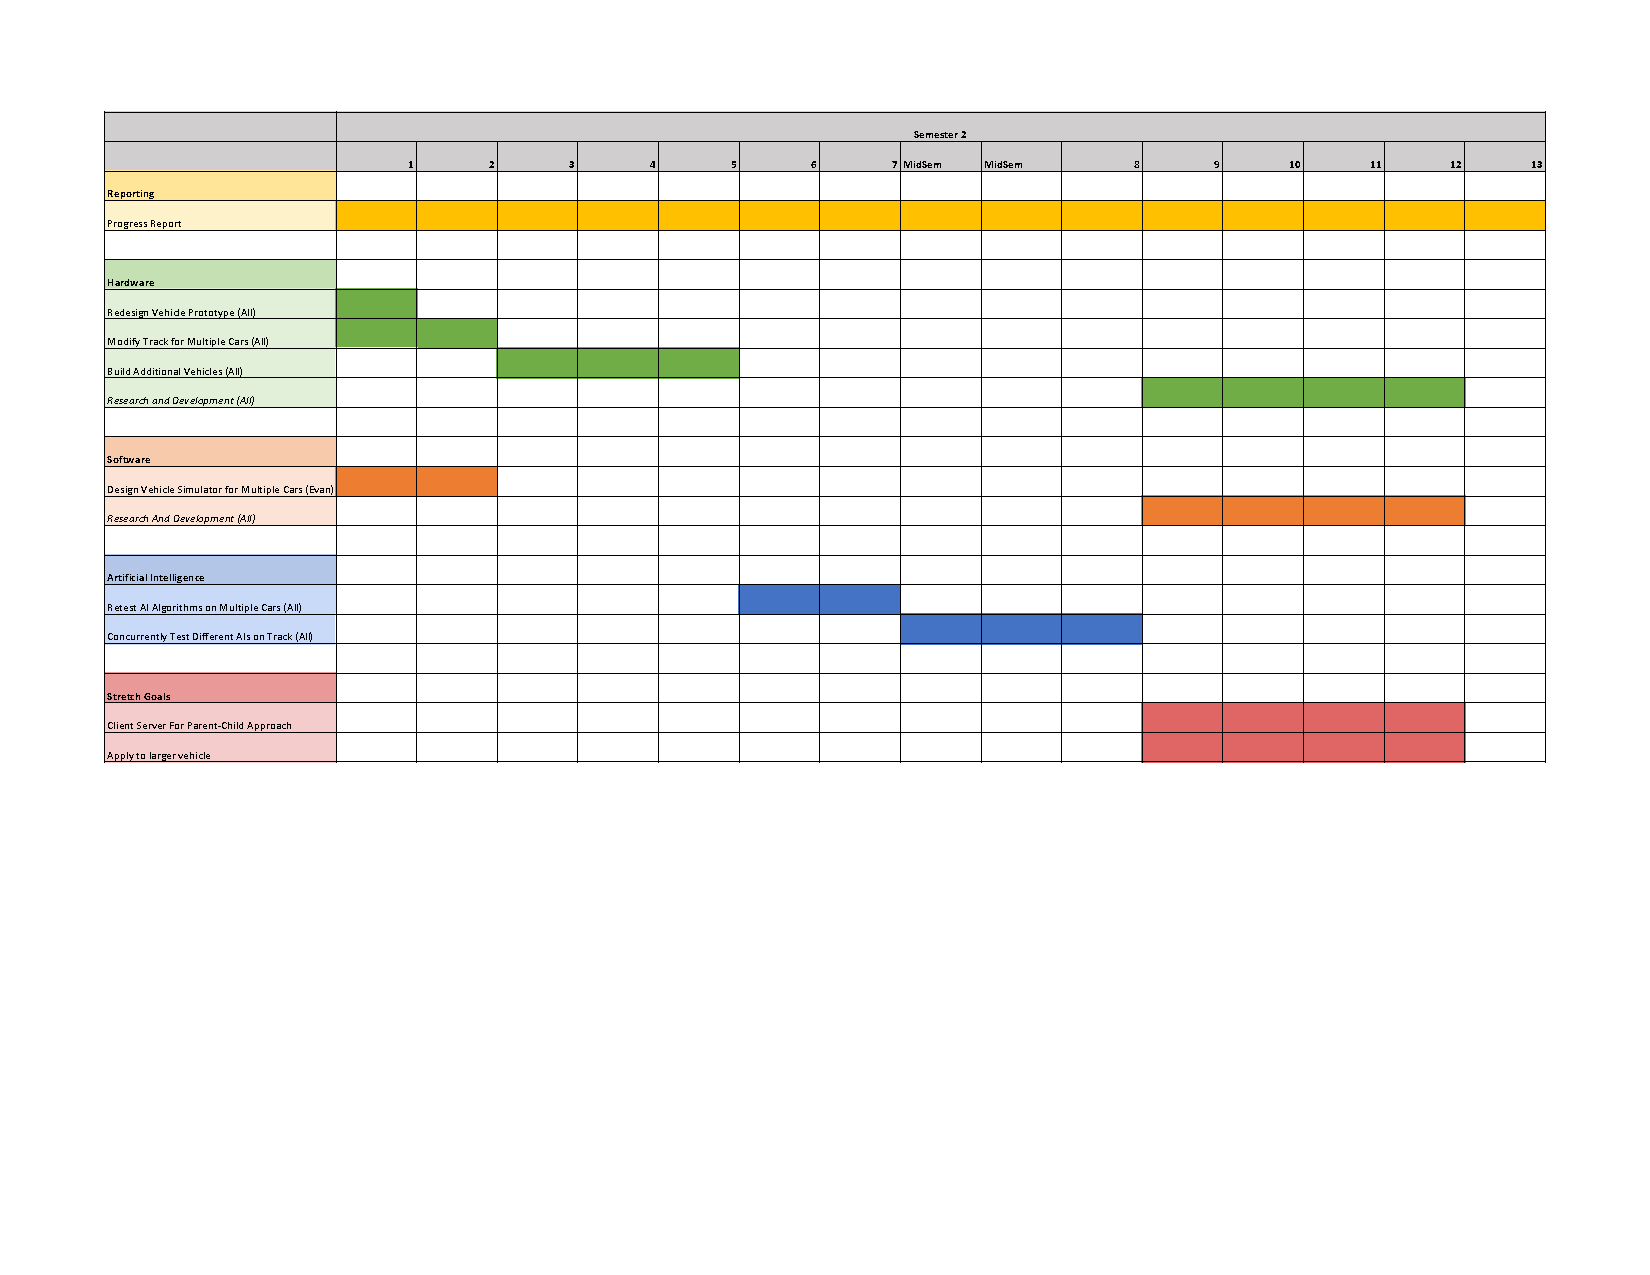
\includegraphics[width=23cm, height = 20cm, angle=90]{figures/TimelineSem2_2.pdf}
	\caption{Expected Timeline for Semester 2}
\end{figure}


\newpage



%      %%%  	    %%%  
%     %%%%		   %%%%	
%    %%%%%		  %%%%%	
%   %%%%%%		 %%%%%%	
%      %%%		    %%%	
%      %%%		    %%%	
%      %%%		    %%%	
%      %%%		    %%%	
%      %%%		    %%%	
%      %%%		    %%%	
%   %%%%%%%%%	 %%%%%%%%%
%   %%%%%%%%%	 %%%%%%%%%
%
%
% -----------------------------------------------------------------------------------------------
%

\subsection{Semester 1 Milestones}
\subsubsection{Hardware}
\textbf{Sensor Testing (Mathew)} - Mathew will be conducting individual sensor testing before building the first prototype, giving us background knowledge and determining the best suited sensors. Two weeks will be used to research individual components and determine their benefits.
\\\\
\textbf{Interface RC Vehicle with Raspberry Pi (Mathew)} -The Raspberry Pi will connect with the car's circuitry. Additional time will be allocated for debugging. This milestone should deliver a fast response time and precision control over the vehicle’s motors.
\\\\
\textbf{Design Vehicle Prototype(Mathew/ Jordan)} - The vehicle must be large enough to support a Raspberry Pi, as well as additional components (Breadboard, sensors, wires, etc.) 3D printing is an avenue worthy of exploration for mounting purposes. This small milestone should take less than a week to complete.
\\\\
\textbf{Build Vehicle Prototype (Mathew/ Jordan)} - Following the design and construction, sensors and other required electronics will be mounted to the car (possibly including 3D-printed mounts). This milestone should be able to be completed shortly after designing the vehicle prototype.
\\\\
\textbf{Design Race Track (Mathew / Jordan)} - Our vehicle prototype will need a track to train and improve, constructed out of cheap, sturdy and modifiable materials. Constructing multiple tracks is essential in the training stage, such that the vehicle does not overfit to a specific track. This is a small milestone to complete though must give consideration to the chosen material.
\\\\
\textbf{Build Race Track (Mathew  / Jordan)} - The race track will be assembled at one of the team member’s house. It is planned to test the track with an unmodified RC car to determine the track robustness and difficulty.



\newpage


%      %%%  	    %%%%%
%     %%%%		  %%%%%%%%%
%    %%%%%		 %%%     %%%
%   %%%%%%		         %%%
%      %%%		         %%%
%      %%%		    %%%%%%%
%      %%%		  %%%%%%%
%      %%%		 %%%
%      %%%		 %%%
%      %%%		 %%%
%   %%%%%%%%%	 %%%%%%%%%%%
%   %%%%%%%%%	 %%%%%%%%%%%
%
%
% -----------------------------------------------------------------------------------------------
%
\subsubsection{Software}
\textbf{Model Car (Evan)} - Accurately model the RC car for use in the simulation.
\\\\
\textbf{Design Simulator / Track Editor (Evan)} - Designing and creating a real world simulation with the Unity\cite{Unity3D} Game Engine, including track editor, for testing and simulating the physics of the car, and the implementations of the AI algorithms.
\\\\
\textbf{Sensor Simulation (Evan / Jordan)} - The functionality of the sensors we will be using should be accurately simulated to ensure the AI performs similarly to the real world counterpart.
\\\\
\textbf{User Interface(UI) (Mathew)} - A main menu screen will welcome users to the software. The design must be minimal and clear for users to interpret. Two weeks will be used to draft an interface and improve features at a later date.
\\\\
\textbf{Combine UI, Simulator, Track Editor (All)} - Combining independent software programs into one main package. The Main Menu will link to the Track Editor or Car Simulator. This milestone should be completed very quickly if everything performs as expected.
\\\\
\textbf{Implement AI Algorithms (Evan, Jordan)} - Implement Condition Based (1 week), Evolutionary(3 weeks), Q-Learning (2 weeks)\cite{QLearningRobotControl} and Deep Q-Learning\cite{DeepQLearningReleasePaper} (2 weeks) algorithms.



\subsubsection{Combination}

\textbf{Apply Conditional Based AI to RC Car (All)} - The team will be applying the Conditional Based AI to the physical car. Due to the simplicity of this milestone, it should be completed within a week.
\\\\
\textbf{Apply Chosen AI to RC Car (All)} - After running all AIs in the software simulation, the best AI will be applied to the RC car. Two weeks will be used to test other AIs on the RC car, allowing enough time for the Evolutionary Algorithm to be fairly tested. 
\\\\
\textbf{Test and Tweak AI (All)} - If an AI is not performing as expected once applied to the RC Car, the team can tweak the AI to improve performance. The lead-up weeks to the end of the first semester will be used for this milestone.

\subsection{Project Feasibility}
In terms of feasibility, this project will include challenges for all team members. Though there are many complex tasks involved in this project, it is believed that the semester 1 timeline  is realistic and achievable. There is also an option to push certain milestones into the second semester (though this is not ideal).

\newpage

\section{Ethics Considerations}
There are little to no ethics clearances required, though there are still some ethical considerations to examine.
\\\\
Due to the size of the RC Car, it will not cause any hazards or damage to humans or property in the event of an ‘accident’. The vehicle will hold a Raspberry Pi, sensors and various cables that will be secured properly. The car will not be able to leave the track during operation due to barriers. 
\\\\
Data is planned to be gathered from ultrasonic sensors, meaning that there will be no need for human interaction or human consent of data.

\section{Statement of Individual Contribution}
All team members were involved in the process of creating a title and writing a summary.
\\\\
\emph{Mathew} wrote the Background section outlining the reason why the team decided to complete a project on this topic. Mathew also wrote about the approach the team will take to complete the project.
\\\\
\emph{Evan} wrote about the Aims and Expected outcomes in the project. This provided a plan on how to achieve the expected goals for this project. Evan is the most experienced with Artificial Intelligence and is taking a managerial position to expand his skillset.
\\\\
\emph{Jordan} wrote the Activity Plan / Timetable section. Each group member was involved in designing the Gantt Charts for Semester One and Semester Two, allocating assigned tasks to be completed. Jordan expanded on each Gantt Chart milestone, explaining what must be achieved to complete the milestone. Jordan wrote about the ethical considerations and formatted the document in Latex.


\newpage



%      %%%   	    %%%%%
%     %%%%	 	  %%%%%%%%%
%    %%%%%	 	 %%%     %%%
%   %%%%%%	 	 %%%     %%%
%      %%%	 	 %%%     %%%
%      %%%	 	    %%%%%
%      %%%	 	 %%%%%%%%%%
%      %%%	 	 %%%     %%%
%      %%%	 	 %%%     %%%
%      %%%	 	 %%%     %%%
%   %%%%%%%%% 	  %%%%%%%%%
%   %%%%%%%%% 	    %%%%%
%
%
% -----------------------------------------------------------------------------------------------
%



%code example
%\vspace{10pt}
%\begin{lstlisting}
%    #include <iostream>
%    using namespace std;
%
%    int main() {
%    	cout << "Hello World" << endl;
%    	return 0;
%    }
%\end{lstlisting}
%\vspace{5pt}




%
% ---- BIBTEX STUFF -----------------------------------------------------------------------------
%\bibliographystyle{plain}

\bibliography{COMP3851AProjectPlanReport}
\bibliographystyle{ieeetr}

% -----------------------------------------------------------------------------------------------
%

\end{document}